\section{Ensamble learning}
Si fanno tante predizioni e poi si combinano.

\begin{figure}[H]
    \centering
    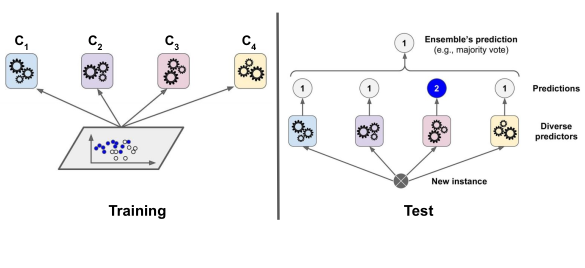
\includegraphics[width=0.8\linewidth]{imgs/ensemble-learning}
    \caption{Ensemble learning}
    \label{fig:Ensemble_learning}
\end{figure}

Se ho tanti classificatori, posso ripetere la classificazione su tatnti modelli diversi
con i corrispettivi errori(\textbf{indipendenti fra loro}).

Ho modo di aumentare la probabilità di prenderci se i modelli che uso
sono separati fra di loro, e le decisoni quindi non sono condizionate
dagli altri modelli.

\subsection{Bootstrap aggregating(Bagging)}
Se ho un solo dataset, porto ai modelli comunque lo stesso dataset con gli stessi
errori comuni, uso la tecnica di \textbf{bootstrapping} dove porziono il dataset
in sotto sezioni e assegno diverse sezioni a diversi modelli,
cosi da eliminare anche i problemi legati ai dati simili.

\subsection{Random forest}
È un mmodello bagging dove fa l'aggregazioni di alberi decisionali.

\subsection{Hard voting classifier}
Usare algoritmi diversi con classificatori diversi e poi fare un hard voting
\textbf{codice di pag 22 cap 13 figo}

\subsection{Boosting}
Simile al bootstrapping ma fatto in maniera sequenziale(l'output di uno è l'input del successivo).

Ogni predizione cerca di correggere la precedente.

\subsubsection{AdaBoost}
\begin{itemize}
    \item per correggere il predecessore, presta attenzione alle istanze del training
    che il predecessore ha underfittato
    \item il nuovo "predittore" si concentra di più sul hard case(adaptive)
    \begin{enumerate}
        \item La prima predizione è treinata e usata per fare predizioni sul training
        \item I pesi di missclassification vegono incrementati
        \item la seconda classificazione usa i pesi aggiornati
        \item Ad ogni classificatore viene assegnato un peso
        \item Dopo che ogni "predicter" ha finito il train, viene fatta unapredizone come nel
        bagging, tranne per il fatto che le predizioni hanno un peso.
    \end{enumerate}
\end{itemize}

\begin{figure}[H]
    \centering
    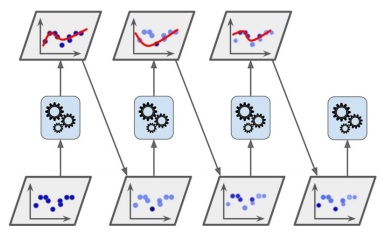
\includegraphics[width=0.3\linewidth]{imgs/ada-boosting}
    \caption{AdaBoost}
    \label{fig:AdaBoost}
\end{figure}

\subsubsection{Algoritmo di AdaBoost}
Ongi istanza ha un peso w,
inizialemnte settato a $\frac{1}{m}$,
dove m è il numero delle osservazioni.
Per ogni predicotr J, viene calcolato un peso di error-rate $r_J$.

\begin{equation}
    r_J = \frac{
        \sum_{i=1, \hat{y}_j^{(i)}\neq y^{(i)}}^{m} w^{(i)})
    }{
        \sum_{i=1}^{m} w^{(i)})
    }
\end{equation}

Poi viene calcolato il peso $\alpha_J$ in base al learningn rate $\eta$.

Più un predittore è accurato e maggiore sarà il suo peso:
\begin{equation}
    \alpha_J = \eta\log\frac{1-r_J}{r_J}
\end{equation}

Se prova a indovinare a caso ($50\%$) avrà valore vicino a 0, se sbagli il più
delle volte, sarà negativo il suo valore.


Dopo di chè i pesi delle istanze vengon aggiornati con:
\begin{equation}
    w^{(i)}
    \begin{cases}
        w^{(i)} \Rightarrow if \hat{y_j}=y(i) \\
        w^{(i)} \exp(\alpha_j) \Rightarrow if \hat{y_j}\neq y(i)
    \end{cases}
\end{equation}

Dopo aver aggiornato tutti i pesi, adaBoost computa la predizione usando i pesi.

La classe predetta è quella che prende la magioranza di voti pesati.

\subsubsection{Gradient Boosting}
La chiave del GB è la additività dei modelli, si puo arrivare ad avere
un imparatore finale:
\begin{equation*}
    F_L=f_0(x) + \dots + f_{L-1}(x)
\end{equation*}

dove la L è il numero di learner che si usano ed f0 è il primo learner che apprende
dal dataset, gli altri learner dopo di lui cercano di migliorare il risultato
riducendo la loss function.

Ogni learner prende il nome di epoch, e durante ogni epoch si cerca di ridurre la
loss e non di aumentare le istanze(come fa adaBoost).



































